\documentclass{report}
\usepackage[utf8]{inputenc}
\usepackage[acronym]{glossaries}
\usepackage{biblatex}
\usepackage[colorinlistoftodos]{todonotes}
\usepackage{graphicx}
\usepackage{pgfplots}
\usepackage{fancyvrb}

\addbibresource{bibliography.bib}


\title{Detekt-hint -- Detection of design principle violations}
\author{Marius Kohmann}
\date{June 2020}


\newacronym{ast}{AST}{Abstract Syntax Tree}
\newacronym{solid}{SOLID}{\textbf{S}ingle responsibility, \textbf{O}pen–closed, \textbf{L}iskov substitution, \textbf{I}nterface segregation, \textbf{D}ependency inversion}
\newacronym{dry}{DRY}{Don't Repeat Yourself}
\newacronym{srp}{SRP}{Single Responsibility Principle}
\newacronym{ocp}{OCP}{Open-Closed Principle}
\newacronym{lsp}{LSP}{Liskov Substitution Principle}
\newacronym{isp}{ISP}{Interface Segregation Principle}
\newacronym{dip}{DIP}{Dependency Inversion Principle}
\newacronym{lcom}{LCOM}{Lack of Cohesion Of Methods}
\newacronym{loc}{LOC}{Lines Of Code}
\newacronym{mvvm}{MVVM}{Model-View-ViewModel}
\newacronym{pr}{PR}{Pull Request}
\newacronym{ntnu}{NTNU}{Norwegian University of Science and Technology}
\newacronym{mimc}{MIMC}{More Is More Complex}
\newacronym{kiss}{KISS}{Keep It Simple Stupid}
\newacronym{psi}{PSI}{Program Structure Interface}
\newacronym{dsm}{DSM}{Dependency Structure Matrix}
\newacronym{lod}{LoD}{Law of Demeter}
\newacronym{qa}{QA}{Quality Assurance}

\begin{document}

\maketitle

\begin{abstract}
	%Sample IMRaD abstract: 
	Absence of correctly applied design principles triggers maintainability problems in software development and increases development cost. A tool for identification of design principle violations were developed using the design science methodology. The product was evaluated by testing on others code, using horizontal prototypes and having a workshop testing the product. 
	
	
	
\end{abstract}


\clearpage
\tableofcontents
\clearpage
\chapter{Introduction}

% Why maintainable code is important
Writing maintainable and high quality code is an important part of software engineering. Various people define software maintainability differently, but a commonly accepted collection of quality attributes include extensibility, modularity, testability and understandability. To help developers write code with those attributes, well defined rules and conventions have been developed. They are often enforced by the use of tools commonly referred to as linters. Design principles is another invention that has been created to help developers write code that adheres to the aforementioned quality attributes. Unfortunately, many of the principles are not formal and is often open for interpretation and subject for debate. Therefore, correct appliance of the principles often requires reasoning about the business domain and predicting future changes to the code base. The absence of correctly applied design principles triggers maintainability problems and is often a breeding ground for bugs, refactoring\footnote{From Wikipedia: Process of restructuring existing code without changing its external behavior \cite{refactoring}.} tasks and technical debt\footnote{From Wikipedia: Concept in software development that reflects the implied cost of additional rework caused by choosing an easy (limited) solution now instead of using a better approach that would take longer \cite{technicalDebt}.}. Consequences include increased development time, inaccurate estimations causing lost deadlines and higher costs of introducing new developers to the project.

Code analysis using tools, and code review are two techniques used for detecting design issues or design principle violations in code. According to a pre-study on the current state on tools for improvement of code quality-study \cite{prestudy}, current tools are giving limited options for detecting design issues in code, and manual code reviews suffers from human failure.  \todo{sources that can help me argue that code review don't pick up everything.} By combining code analysis and manual code review the primary objective of the study is to see whether we can detect more design issues. Using the design science methodology an innovative product will be developed through short iterations that includes the use of prototypes and continuous feedback. The study will present the inner workings of the product as well as a detailed evaluation of the final artifact.

 %More specifically we will study which design principles that are eligible for code analysis and code review, how to reduce the amount of false-positives and how violations can be reported back to the developer.  


%Some tools offer analysis for detection of some design principle violations, but they suffer from false-positives and not being integrated into the development process - resulting in a high degree of context switching. 

% Code review
%Manual process of inspecting code are error-prone, suffers from "large pr syndrome" and the fact that different developers apply the design principles differently.


The outline of the paper is as follows; Section \ref{background} gives some background information and an introduction to the topics of writing code with high quality and code analysis. Section \ref{methodology} describes the methodology of the research process. Section \ref{relatedwork} gives some insight in related work in the area and section \ref{results} presents the developed artifact, and a detailed evaluation of it. Section \ref{discussion} discusses the results, and lastly in section \ref{conclusion} we conclude the study.  

\chapter{Background}
\todo{watch out for self-plagiat. Diff with the pre-study when things starting to get fininished - smooth checker: https://copyleaks.com/compare .}
\label{background}
To see why achieving maintainable code is so important, and why a new tool for detecting design principle violations is suggested, we need some background information on what maintainable code is and how we can achieve it. The following sections will give a brief introduction to it.

\section{What is maintainable code?}
Software is a product that evolves over time and that continuously needs, fixes, features and updates according to the customer and users needs. To make the process of developing and maintaining a software product cheapest we need to ensure it meets certain requirements regarding quality. The software community is highly opinionated and software quality is measured differently based on (but not limited to) domain, programming language and business requirements. Therefore, measuring software quality and creating rules without exceptions is extremely hard. However, what we know is that the ratio of time spent reading versus writing code is well over 10 to 1 as Robert C. Martin states in \cite{Martin:2008:CCH:1388398}.

To reduce the amount of time spent on reading code (i.e understanding code), we need to ensure that the written code is understandable. We need to ensure that it is easy to understand what the code does and why it does what it does. It should be easy to locate what needs to change, easy to make changes and easy to ensure that the changes does not create unwanted side effects. \hfill 
\hfill \newline

More formally, developers have defined a set of quality attributes that will help ensure that the code is of high quality. A commonly accepted collection of quality attributes include extensibility, modularity, testability, understandability, performance, reliability and security. Martin Fowler did a useful distinction using the terms \textit{internal attributes} and \textit{external attributes} \cite{internalExternal}. The distinction is whether the attribute is visible for the user or customer. The internal quality attributes correspond to maintainability, that is our focus. 

Following are the definitions of the internal quality attributes with most importance in this study:
\begin{itemize}
	\item Extensibility - "Extensibility is a measure of the ability to extend a system and the level of effort required to implement the extension. Extensions can be through the addition of new functionality or through modification of existing functionality. The principle provides for enhancements without impairing existing system functions." \cite{Extensib83:online}
    	\item Modularity - "Modular programming is a software design technique that emphasizes separating the functionality of a program into independent, interchangeable modules, such that each contains everything necessary to execute only one aspect of the desired functionality." \cite{Modularp60:online}
	\item Testability - "Software testability is the degree to which a software artifact supports testing in a given test context. If the testability of the software artifact is high, then finding faults in the system (if it has any) by means of testing is easier." \cite{Software40:online}
	\item Understandability - "Understandability is defined as the attributes of software that bear on the users' (programmer) efforts for recognizing the logical concept and its applicability." \cite{Understa26:online}
\end{itemize}

In the next section we will look into methods of fulfilling these quality attributes.

\section{Achieving maintainable code}
To write code that is maintainable a set of concepts, principles and conventions including; Architectural patterns, design patterns, anti-patterns, design principles, metrics and best practices is used amongst developers. Some of them are well defined, and can easily be verified through source code analysis. Others are more abstract in nature and requires reasoning from the developers and is harder to verify.

An \textit{architectural pattern} is a general, reusable solution to a commonly occurring problem in software architecture within a given context \cite{architecturalpattern}. An example is the \gls{mvvm}-pattern for mobile development \cite{mvvm}. It is a well defined pattern and correct use or misuse could be verified through testing tools like ArchUnit \cite{archunit}. 

A \textit{design pattern} is similar to an architectural pattern, but more limited in scope. An example is the Adapter pattern \cite{Adapterp54:online}. Detection of design patterns is possible through mining \cite{TEKIN2014406}. The absence of patterns is harder to detect as the absence of a design pattern is not clearly defined.

Definitions of \textit{architectural anti-patterns} and \textit{design anti-patterns} have also been made. They are the exact opposite of architectural-patterns and design-patterns. In other words ways one should not solve a common problem. They are often called architecture-smells and design-smells. An example of architectural anti-pattern is the Cyclic Dependency \cite{cyclicdependency} and could be detected through dependency analysis. An example of design anti-pattern is the God-Object \cite{Godobjec14:online}, and is as stated about design patterns, not easily verifiable. However, metrics such as a high value of coupling and \gls{loc} could imply possible violations.


\textit{Design principles} are a set of guidelines that programmers should follow to avoid bad design. Because the design principles is of most importance in this study, a more in depth description is provided in section \ref{design-principles}.

\textit{Metrics} have been developed to measure how well one adheres to the design principles. Examples include cyclomatic complexity and coupling. \textit{Coupling} is the degree of interdependence between software modules \cite{Coupling2:online}. \textit{Cyclomatic complexity} is used to indicate the complexity of a program \cite{Cyclomat54:online}. They are easily calculated using code analysis.

\textit{Best practices} are informal rules that have been learned over time, or practice that have become part of the language ``culture''. The best practices can in some ways be equal to the design principles, but are often simpler and more limited in scope. Even if limited in scope, the range of different best practices is huge. Best practices includes but is not limited to, code patterns that are probable bugs, styling of code and readability. An example of best-practice in the Java language could be to use camel case (camelCase) \cite{camelcase} on variable-names, or to not have empty else-blocks. They are well defined and are verified using code analysis tools like SonarQube \cite{sonarqube}.

\section{Design principles}
\label{design-principles}
Design principles, also commonly referred to as programming principles, are a set of guidelines that programmers should follow to avoid bad design. According to Robert C. Martin \cite{robertcmartinprinciples} there are three characteristics of bad design that the design principles will help reduce:

\begin{enumerate}
	\item Rigidity - It is hard to change because every change affects too many other parts of the system.
	\item Fragility - When you make a change, unexpected parts of the system break.
	\item Immobility - It is hard to reuse in another application because it cannot be disentangled from the current application.
\end{enumerate}
A common set of design principles that often is referred to is the \gls{solid} principles \cite{solid}.

\begin{itemize}
    \item \gls{srp} -- "... states that every module or class should have responsibility over a single part of the functionality provided by the software, and that responsibility should be entirely encapsulated by the class, module or function." \cite{srp}
    \item \gls{ocp} -- "... states "software entities (classes, modules, functions, etc.) should be open for extension, but closed for modification"; that is, such an entity can allow its behaviour to be extended without modifying its source code." \cite{ocp}
    \item \gls{lsp} -- "Objects in a program should be replaceable with instances of their subtypes without altering the correctness of that program." \cite{lsp}
    \item \gls{isp} -- "... states that no client should be forced to depend on methods it does not use." \cite{isp}
    \item \gls{dip} --  "... states: \newline A. High-level modules should not depend on low-level modules. Both should depend on abstractions (e.g. interfaces). \newline
B. Abstractions should not depend on details. Details (concrete implementations) should depend on abstractions." \cite{dip}
\end{itemize}
    
As you can see, the design principles are often abstract and verification requires knowledge and reasoning about the business domain. For example, referring to the \gls{ocp}, how do you know what is going to be changed in the future, and how are you then going to design for extension? Making classes closed for modification of all changes is impossible and would clearly break the \gls{kiss} principle. And in case of \gls{srp}, how would you determine what is a single responsibility? 

To make matters worse; \gls{dip} suggests introducing abstractions to decouple software modules, while \gls{mimc} principle and \gls{kiss} principles says that introducing abstractions (e.g interfaces, abstract classes) introduces unwanted complexity.

The design principles are therefore hard to verify using code analysis. However, some principles are easier to verify than others, and signs of violation could be detected using code analysis or during code review which is described in section \ref{code-review}.

\section{Code analysis}
\todo{rewrite this to fit programming principles and PSI}
%Using code analysis and analyzing for design principles we can achieve maintainable code, which causes less rework and less context switches. 
To help developers of software systems adhere to the aforementioned concepts, principles and conventions, tools for code analysis have been developed. In code analysis we differentiate between two types of code analysis, dynamic code analysis and static code analysis. \textit{Dynamic code analysis} is done by analysing programs being executed on a processor, while \textit{static code analysis} is purely based on analysis of the source code. Since dynamic analysis is based on program execution it has the advantage of being able to measure the actual CPU, memory and energy performance of the application. 

%It can also gather information about the system that would be hard to detect using static code analysis. Examples include discovery of dynamic dependencies using reflection, or actual application usage. However, that does not mean that static code analysis is not able to target performance or dynamic aspects of source code.

As we search to improve the source code, we have chosen to focus on static code analysis. The static analysis is done by parsing the source code, creating an \gls{ast} and then analyzing the tree for violations of the aforementioned principles, concepts and conventions. Figure \ref{fig:ast} shows a simple example \gls{ast} where a static analysis tools could detect that the expression \texttt{x == 1} always evaluates to \texttt{true} and that the variable \texttt{y} is never used. The tool could then suggest that the branching is unnecessary and that the \texttt{y} variable is removed.  

\begin{figure}[h!]
	\centering
	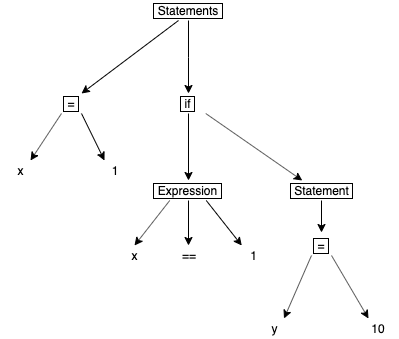
\includegraphics[width=\linewidth/2]{report/images/ast.png}
	\caption{Simple \gls{ast} of x=1; if (x == 1) \{y = 10;\}}
	\label{fig:ast}
\end{figure}

In case of detekt-hint, to do analysis of the Kotlin \gls{ast} easier, Jetbrains\cite{jetbrains} have created an Open-Source \gls{psi} on top, adding utility methods for \gls{ast} analysis and modification. Figure \ref{fig:psi} shows a simplified example \gls{psi} that detekt-hint would use to find violations of \gls{isp}. The analysis would simply look in the PSI for classes that implement interfaces, and see if the overridden methods of that interface are empty or only throws exceptions. 

\begin{figure}[h!]
    \centering
    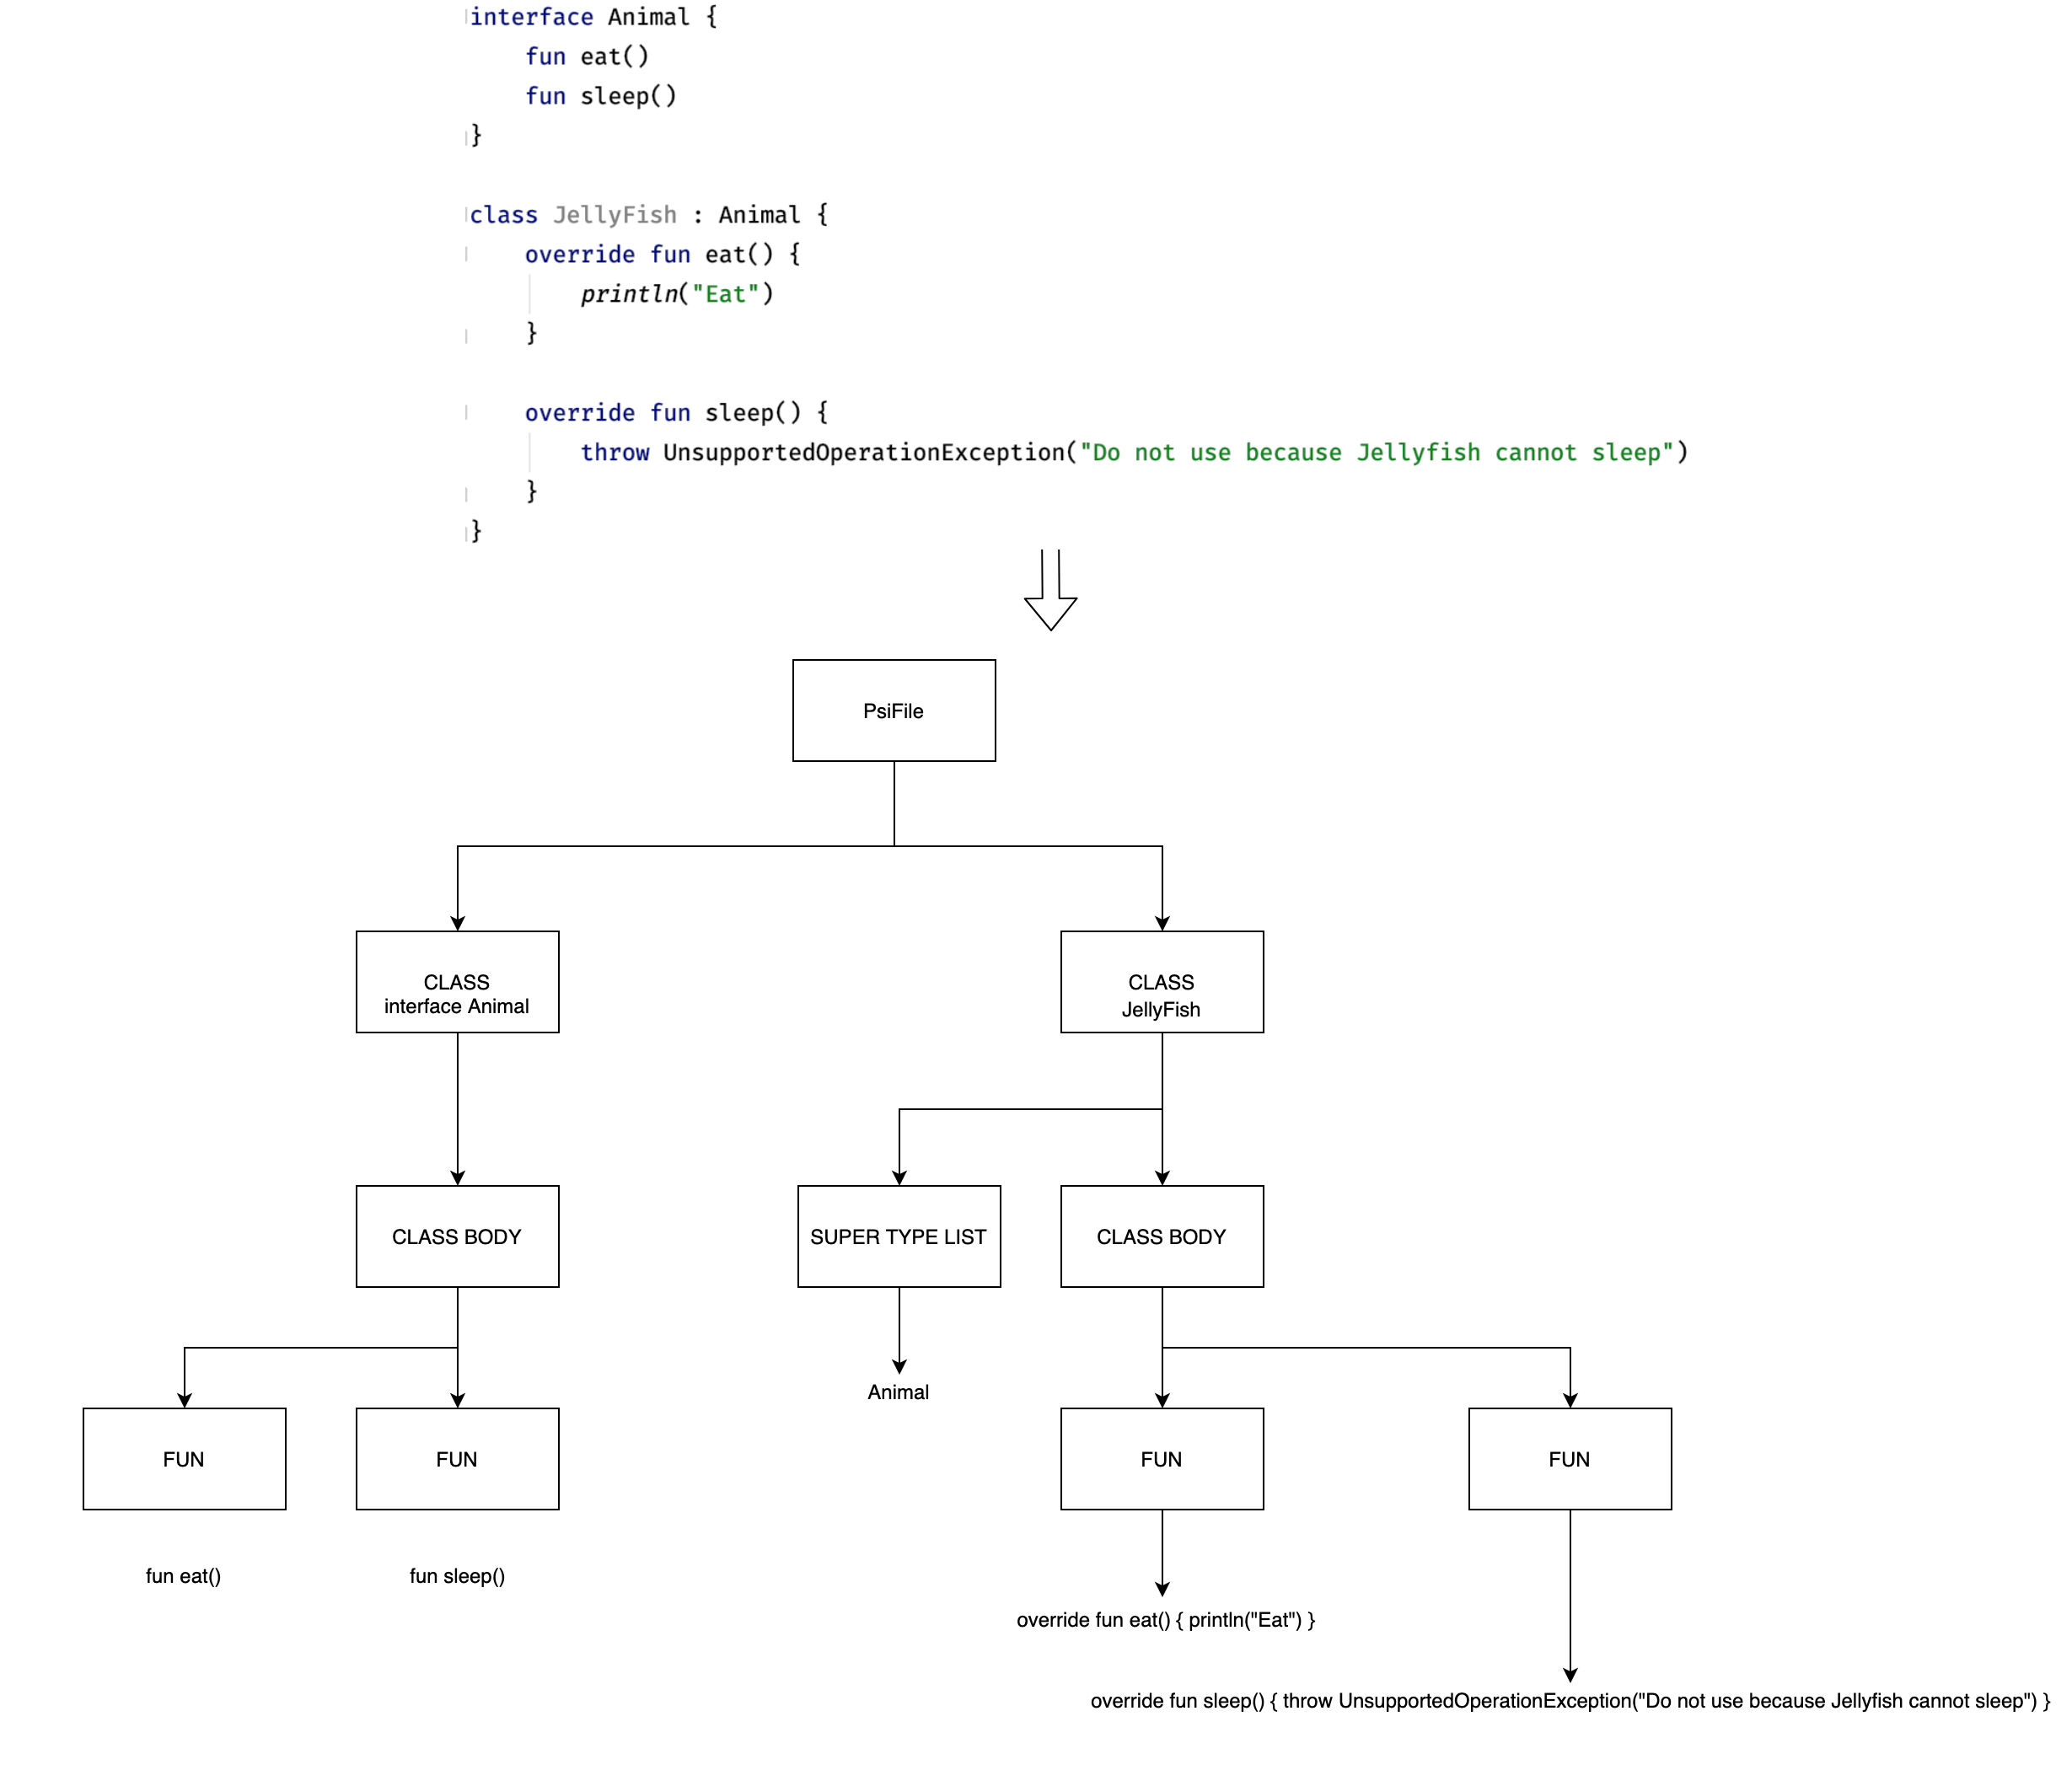
\includegraphics[width=\linewidth]{report/images/psi.png}
    \caption{Simplified version of a sample \gls{psi} showing a sign of violating the \gls{isp}}
    \label{fig:psi}
\end{figure}




\section{False positives and false negatives}
As stated above, most of the design principles are hard to detect violations of. Because we are not totally sure that sure that a design principle is violated and should be our tool will report violations, that isn't. We call these \textit{false-positives}. \todo{add a sample?}We often discuss the rate of false-positives, which is an important metric to evaluate the usefulness of different rules.

A \textit{false-negative} is when actual violation goes undetected. \todo{add sample?}


\section{Code review}
\label{code-review}
Code review is a manual inspection process of looking through code. It is the most common way of finding design issues in code. Code review works very well if done correctly, but unfortunately it is easy get wrong, and is time consuming. 
% why it is easy to get wrong

It is a whole lot of things to consider when doing a code review. Naming a few;

\begin{itemize}
    \item Is the solution well architected?
    \item Will changes cause unexpected behaviour? 
    \item Is the code understandable? Does all variables, method names, classes express its intent?
    \item Is duplicate code introduced?
\end{itemize}

When dealing with large amounts of changed code it is easy to forget some of these. Especially when dealing with repetitive tasks its easy to overlook issues. Tools should therefore help us by automating the most repetitive tasks, such that the time used is focused on finding real design issues. If we can find issues at the time of \gls{qa} the issue will be resolved much quicker because the developer does not need to context switch.

\section{Context switching}
When developing, switching tasks is time consuming. 

\begin{quote}
    ``The trick here is that when you manage programmers, specifically, task switches take a really, really, really long time. That’s because programming is the kind of task where you have to keep a lot of things in your head at once. The more things you remember at once, the more productive you are at programming. A programmer coding at full throttle is keeping zillions of things in their head at once: everything from names of variables, data structures, important APIs, the names of utility functions that they wrote and call a lot, even the name of the subdirectory where they store their source code. If you send that programmer to Crete for a three week vacation, they will forget it all. The human brain seems to move it out of short-term RAM and swaps it out onto a backup tape where it takes forever to retrieve.'' \cite{human-context-switching}
\end{quote} 
If you exchange send to "Crete for three weeks" by fixing design issue (that needs to be resolved for further development) that was introduced one year ago, we can imagine the time to get into that context and resolving the issue. Or imagine maintaining a badly built software project that another group of developers built.


\section{Design science}
Design science is a research methodology that focuses on getting knowledge through development of innovative artifacts. The methodology provides specific guidelines for evaluation and iteration in research projects.

https://medium.com/@pello/design-science-research-a-summary-bb538a40f669
\todo{insert image of design science methodology}

\subsubsection{Prototyping}

horizontal and vertical prototypes. high and low res prototypes.
Used a prototype of the horizontal prototype to verify if i got feedback on what i wanted to. (Test on Eirik)


\chapter{Related work}
\label{relatedwork}
To the best of my knowledge, a tool that only focuses on detecting violations of design principles does not exist. However, some tools and linters include functionality for detecting violations on a small amount of the design principles. I will elaborate on how the different tools support design principles below.

\textbf{High Cohesion - Low Coupling} is a metric that has support in multiples tools, including but not limited to JArchitect \cite{jarchitect} and CodeMR \cite{codemr}. JArchitect \cite{jarchitect} includes functionality for visualizing the High Cohesion - Low Coupling metric using a \gls{dsm}. 

\textbf{\gls{srp}}
JArchitect uses the \gls{dsm} to find violations of \gls{srp} by looking at how many different types a class uses. Ndepend \cite{ndepend} calculates the \gls{lcom} value to find whether the class is cohesive or not, and possibly breaking \gls{srp}. 

\textbf{\gls{lod}}
IntelliJ \cite{IntelliJ} (for Java) has support for detecting violations of the \gls{lod} principle.

\textbf{\gls{dry}}
Detecting similar snippets of code to find violations of the \gls{dry} principle is targeted by many tools including, but not limited to IntelliJ, PMD and Code Climate. However, code can violate \gls{dry} without looking similar, and tools that can detect such issues have not been found.  




Problem being that some of the tools only include a small subset of the principles, making developers need to adopt a large suite of tools to only be able to support detection of violation of design principles.

can be used to find where to start reducing technical debt, but is not highly integrated into the development process 

The problem is that very few tools for detecting design principle violations exists. As mentioned in \ref{relatedwork}, the existing tools analyze the whole codebase and is not integrated with the development process. Using the existing tools can be good for project level analysis activities, and finding areas of improvement. The tools also lack support for many import design principles.

\chapter{Methodology}
\label{methodology}
This study will follow the Design Science methodology which is presented in (A Design Science Research Methodology for Information Systems Research) \cite{10.2753/MIS0742-1222240302}. It is selected because it fits the process of building a innovative software artifact. The software artifact will be created through a series of iterations that include the follow activities; problem identification/understanding and motivation, definition of objectives for a solution, design and development, demonstration/testing, evaluation, communication. Figure \ref{fig:designScience} is taken from Peffers. K \cite{Peffers2007ADS} and shows the process of the design science methodology. 

\begin{figure}[h!]
    \centering
    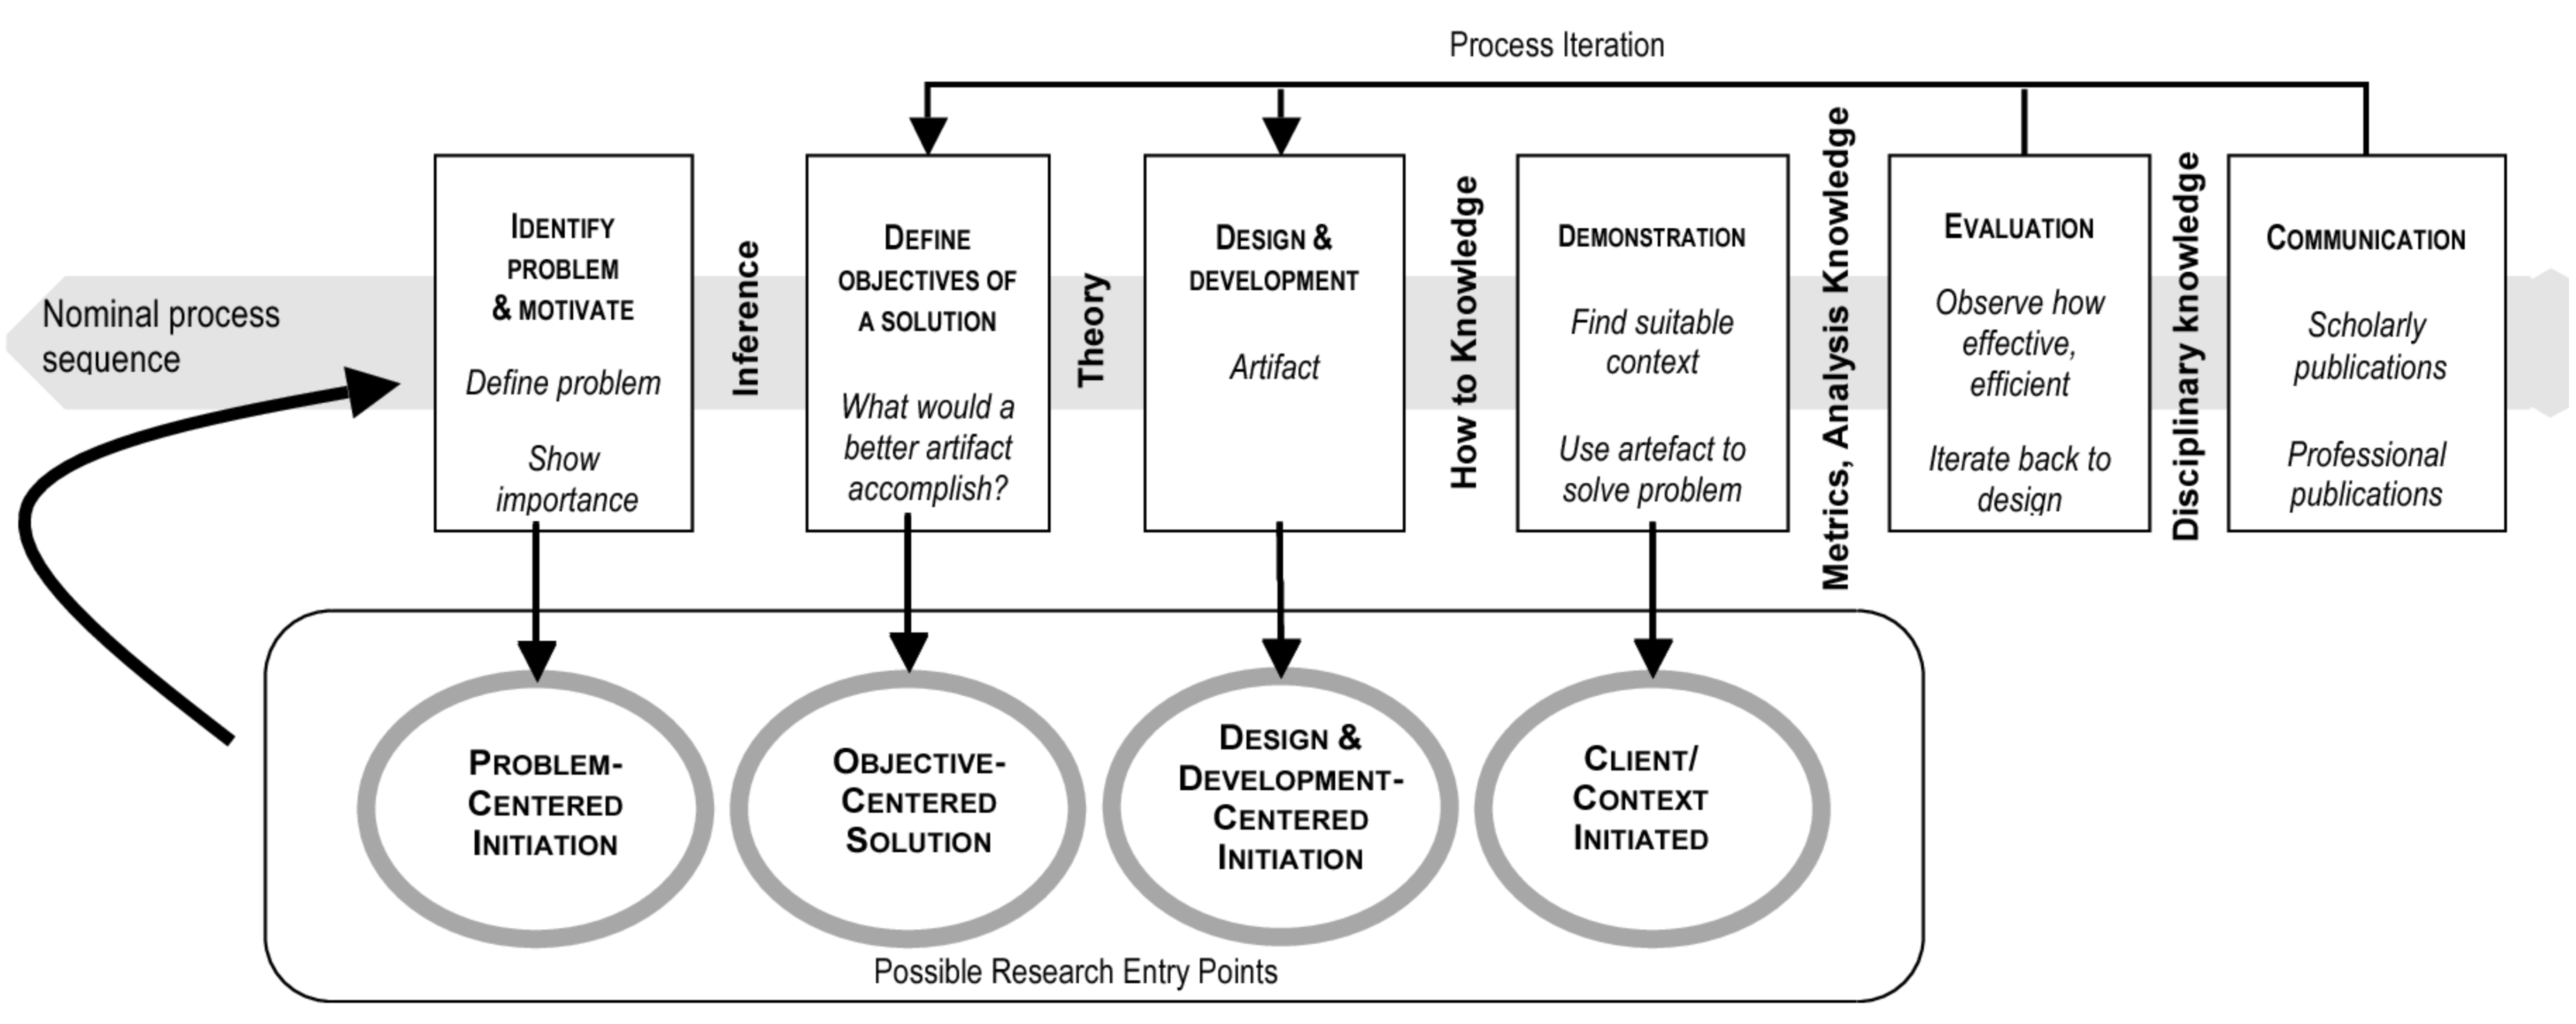
\includegraphics[width=\textwidth]{report/images/designScience.png}
    \caption{The process of the design science research methodology}
    \label{fig:designScience}
\end{figure}



As can be seen in the figure is important to notice that the activities is not done in any particular order, but in that order as seen required. I will elaborate on how the different activities is applied to the project below. 



\section{Problem identification and motivation}
Absence of correctly applied design principles triggers maintainability problems and is often a breeding ground for bugs, refactoring tasks and technical debt. Finding design flaws as soon as possible is a crucial task to limit the amount of rework required. There are mainly two reasons for this: 

\begin{enumerate}
    \item Building upon badly designed software further complicates and increases the difficulty of fixing the software.

    \item The developer is in the context of the current code. Fixing design flaws as soon as possible would require less time to do because the developer knows the context and does not need to context switch.

\end{enumerate}

There are mainly two techniques for detecting design issues, code-analys using tools and manual code-review. Some code-analysis tools offer design principle analysis as mentioned in section \ref{relatedwork}, but suffer from limited functionality regarding design principles and not being integrated into the development process. Therefore, manual code review is the main arena where most design-issues are found. Finding design issues through code review is time-consuming and requires deep understanding of the problem that is being resolved. This process is prone to errors and overlooking due to the nature of human failure. Having a tool that could help this process would help both the reviewer and the reviewee with not overlooking possible design issues, and could cause useful design discussions within the team.

\hfill \newline
This problem identification raises an important question which is my main research question:
\hfill \newline
\hfill \newline
\textbf{RQ1}: How can one use techniques for detecting design principle violations to improve the maintainablity of code? \newline
\textbf{RQ1.1}: Which design principles can be verified using code analysis? \newline
\textbf{RQ1.2}: How to deal with a high rate of false-positives? 


\section{Define objectives of a solution}
\label{objectives-of-solution}
Initially the objectives of a solution had the following chacacteristics:
\begin{enumerate}
    \item It detects violations of important design principles through a set of rules using static code analysis
    \item False-positives should not create too much noise in the developer workflow. First, the rate of false positives should be reduced as much as possible. Second, reported violations should be easy to ignore. 
    \item It contributes to detecting design issues at the time of \gls{qa}.
    \item It should be configurable for defining desired threshold values and turning off unwanted rules
\end{enumerate}

During development it came to mind that reported violations should include context of the code (referring to actual constructs in the code) to ease the process of deciding if a detection is a true- or false-positive. 
\begin{enumerate}
  \setcounter{enumi}{4}
    \item Reported violations includes code context to ease the process of deciding if it is a true- or false-positive. 
\end{enumerate}

Later on, it was discovered that the performance and ease of setup are crucial objectives to make developers adopt the tool. Therefore, two new objectives for a solution was defined:
\begin{enumerate}
\setcounter{enumi}{5}
     \item It is easy to set up and use for all team members in the project
    \item Good performance
\end{enumerate}

%It all boils down to time=\$. The tool will only provide value of we can save development time using it. Then, if the sum of time saved by finding design issues earlier is more than the sum of the negative impact of considering the false-positives, the tool will provide value.
%As a general objective we can say that, the tool will provide value if the value of detecting true-positives is worth more than the negative impact of all the false-positives. 
%However, to measure the time spared by detecting issues earlier is an impossible task to measure, but we know that it is quite


Rule specific objectives: 
Comments are understandable, and provides suggestions for solutions.

\section{Design and development}

Involves the development of the final software artifact and both horizontal and vertical prototypes. Prototypes is used early in the development phases to quickly be able to evaluate the product. Horizontal prototypes should be created to early demonstrate a broad view of the final artifact. Vertical prototypes will be used to elaborate on technical challenges and the workings of specific features. 
 
\section{Demonstration}
Gather people for an workshop and presentation of horizontal prototypes. Important to create a structured schema with questions and impressions to get feedback in a structured way that can be used to evaluate the different features.

Posted on social media to get feedback. Having a presentation for Javabin Trondheim to get informants. Direct contact with friends and possible informants. Posted in slack for work.
 
\section{Evaluation}
Continuous evaluation of the developed artifact is important to adjust the product to the users needs. Multiple evaluation methods were used on different stages of the project, ranging from interest measurement from posts on social media, interviews, semi structured interviews, discussions, presentations and running the program on own and others code.

The following stages of development will be evaluated: 
\begin{itemize}
    \item Idea 
    \item Requirement specification
    \item Development
    \item Presentation of horizontal prototype
    \item Vertical prototype
    \item Final artifact
\end{itemize}


Not all objectives defined in section \ref{objectives-of-solution} will be applicable for all the evaluations.

The results from the evaluations is presented in the result chapter.


\section{Communication}


My needs for this solution. Needs a AST to analysis and a framework to help me with this. Need a way of creating a report of the analysis and feed it to something else that can post on github. 


\chapter{Results}


\section{Evaluation results}
% Not that much focus on creating and hitting bullseye with the product, more about the feedback itself and how to respond to it.

\subsection{Idea}
Ok to reference popularity on github/reddit, but can be misvisende and it is important to not take the response there for god fisk.
Un-structured feedback trough Reddit. However, i posted an image of the MVP on Reddit/Kotlin, and it quickly got so many upvotes that it was top this week in under 12 hours. 

\subsection{Requirement specification}
\subsection{Development}

\subsection{Horizontal prototype}
\subsection{Vertical prototype}
\subsection{Final artifact}
Through a workshop the final artifact was evaluated. Analysis of pull requests and see if we can find some issues.
Schema:
Who is the participants, some background information on them. What did the participants say. What is the takeaway from the workshop? What did i change in the product after having the workshop?

What is the goal, how should i reach the goal of the workshop. Keep the workshop structured.


Gather a group of Kotlin/Android entusiasts for a workshop where one could order pizza and code using this tool. Focus on feedback. Could for example analyze some code that they know and give some feedback on whether it is useful or not. What would have been useful?

\section{Produced artifacts}

\subsection{Horizontal prototype}
The horizontal prototype was built by creating sample \gls{pr} in a sample repository on Github\cite{sample-repository}, and then commenting on the \gls{pr}'s with the bot user. An example from the prototype is presented in figure \ref{fig:liskov}. 

\begin{figure}[h!]
    \centering
    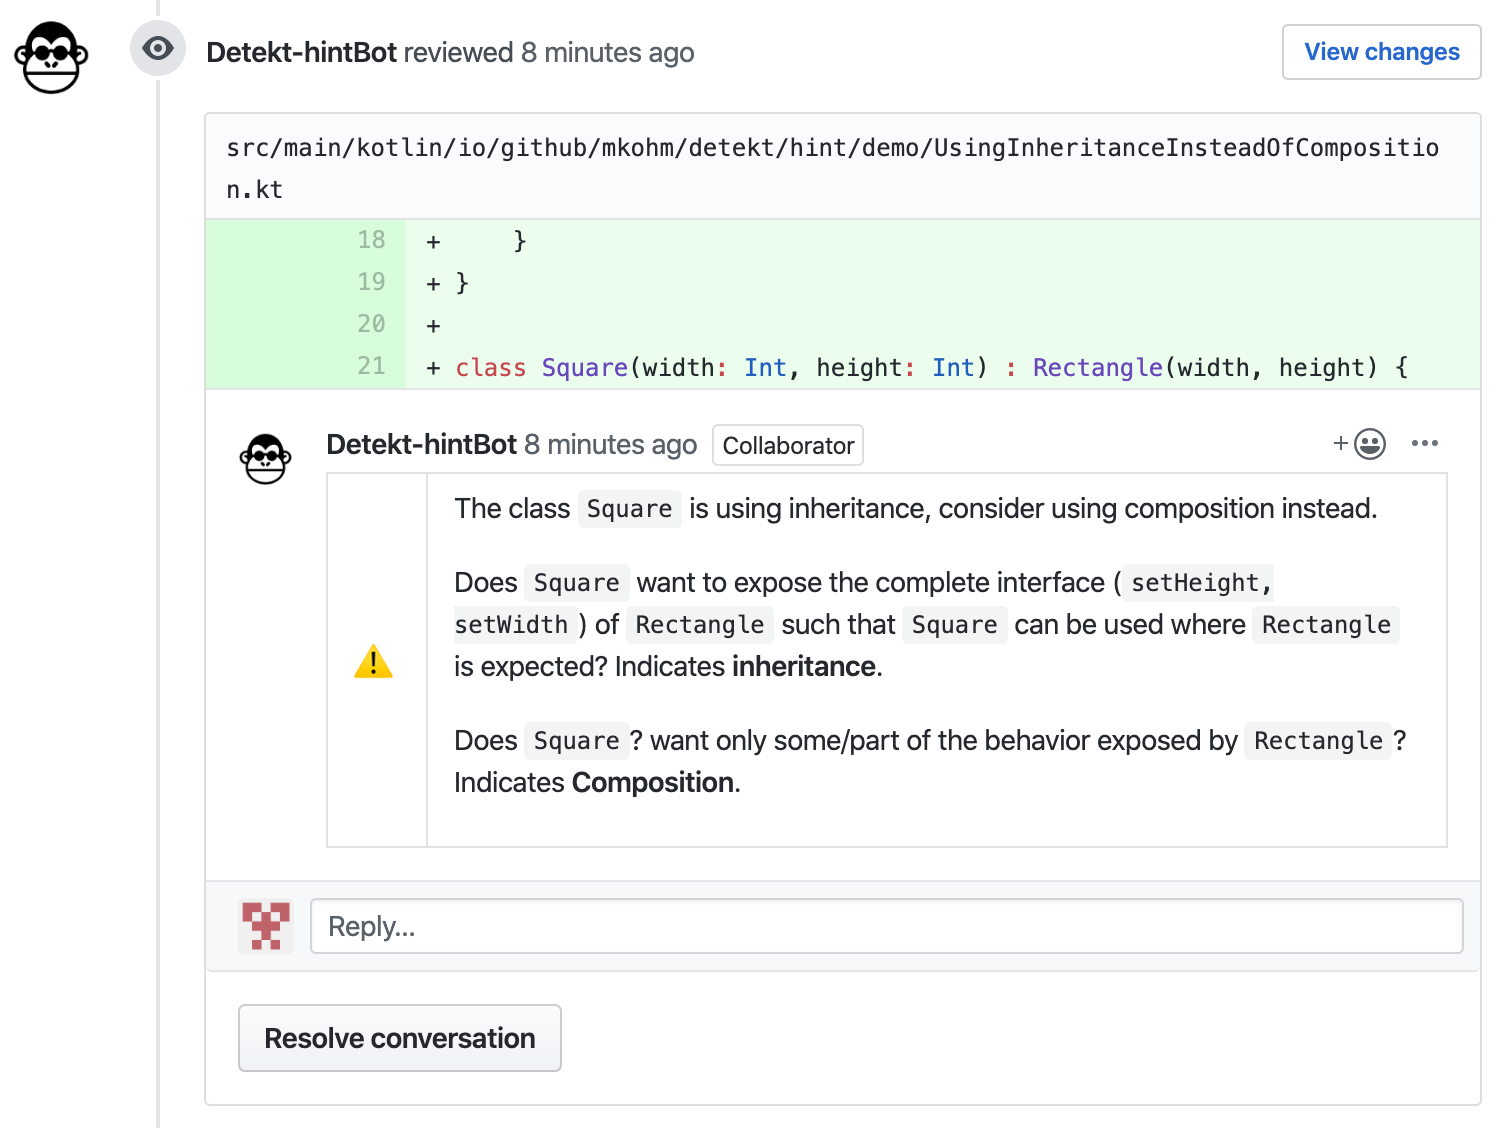
\includegraphics[width=\textwidth]{../demo.png}
    \caption{Prototype of the composition over inheritance / \gls{lsp} rule}
    \label{fig:liskov}
\end{figure}

% What did i find when using this prototype? What changes does the product need, or does it confirm that i am on the right path?

The schema used for the semi-structured interview, the participants answers/feedback and selected images of the prototype can be found in appendix \ref{horizontal-prototype}. The full prototype can be found in the sample repository \cite{sample-repository}. 

\subsection{Vertical prototype}
To get structured feedback on the prototype it 
Horizontal prototypes with github PR samples with bot commented. Was easily created by pushing code to repo and logging in as the bot. Should create samples that demonstrates possible false positives as well as true positives. 

Main takeaway from feedback: 

People think it is an interesting project.
Focus on reducing false-positives.
Does not need a diagram, can use text instead?



Creating a vertical prototype with a simple rule (usecomposition rule) to see if this project it technically possible within the time frame of a masters thesis. 

The schema for the workshop can be found in appendix \ref{workshop-schema}.


\subsection{Detekt-hint specification}
Specification of all the rules.

\subsection{Detekt-hint}

\subsubsection{Architecture}
A diagram of how everything interacts with each other.

\subsubsection{Detekt}
Detekt is a static analysis tool for kotlin. Which provides access to a framework for rule creating for analyzing code and reporting warnings.

Detekt gives us access to IntelliJ PSI for analyzing Kotlin code. The PSI is built on top of the \gls{ast} provided by the kotlin compiler, and provides utility methods for modifying and querying of the underlying \gls{ast}.

Type resolution?

\subsubsection{Detekt-hint}
Final source code can be found on Github\cite{detekt-hint-repository}

\subsubsection{Danger}

\subsubsection{Danger detekt plugin}

\chapter{Discussion and conclusion}
\label{discussion}

\section{Descussion}

\section{Future work}
Implement more rules.
Reducing the amount of false positives.

Providing more context and/or possible solutions in the comments. Images or graphs explaining.
Increasing the performance.
Easing the setup process. Github app? Direct integration with the repository with no setup. A tool like code-climate that does not need any configuration. Plus of tool like this: all setup is in source control. Downside: could be tedious to set up or not all team members want to use it.

\section{Conclusion}
\label{conclusion}

\section{Acknowledgements}
\label{acknowledgements}
Thanks to supervisor, all participants in workshop and prototype sessions.

\printbibliography

\appendix
\label{appendix}
\clearpage
\chapter{Appendix}

\section{Horizontal prototype}
\label{horizontal-prototype-images}

\begin{figure}[h!]
    \centering
    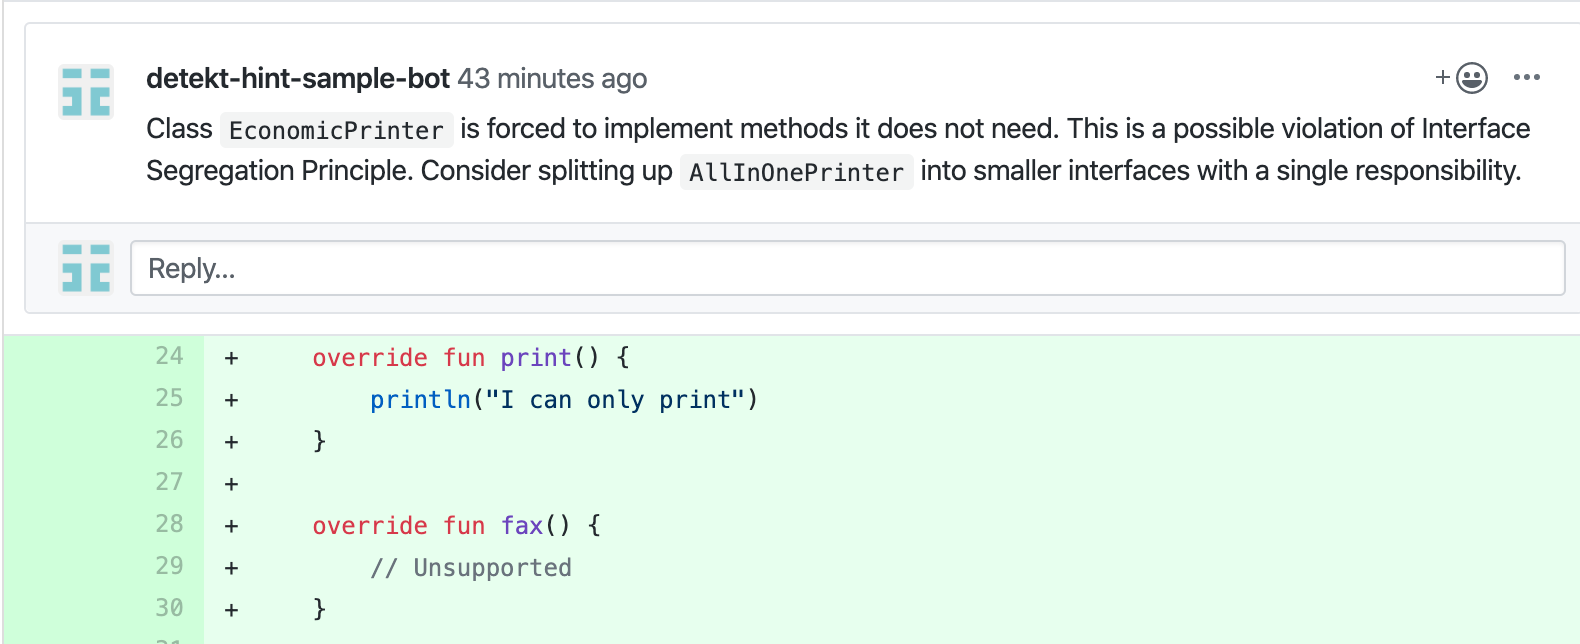
\includegraphics[width=\textwidth]{../images/comment_isp.png}
    \caption{Screenshot of the horizontal prototype showing the \gls{isp} rule. It has detected an empty method, which is a sign of violating the \gls{isp}. In this case the \texttt{EconomicPrinter} implements methods from \texttt{AllInOnePrinter} which it does not need. A solution would be to define separate interfaces for each of the responsibilities (e.g \texttt{Printable, Faxable, Scanable}) and let the concrete implementations of printers implement the interfaces they need.}
    \label{fig:isp}
\end{figure}


\begin{figure}[h!]
    \centering
    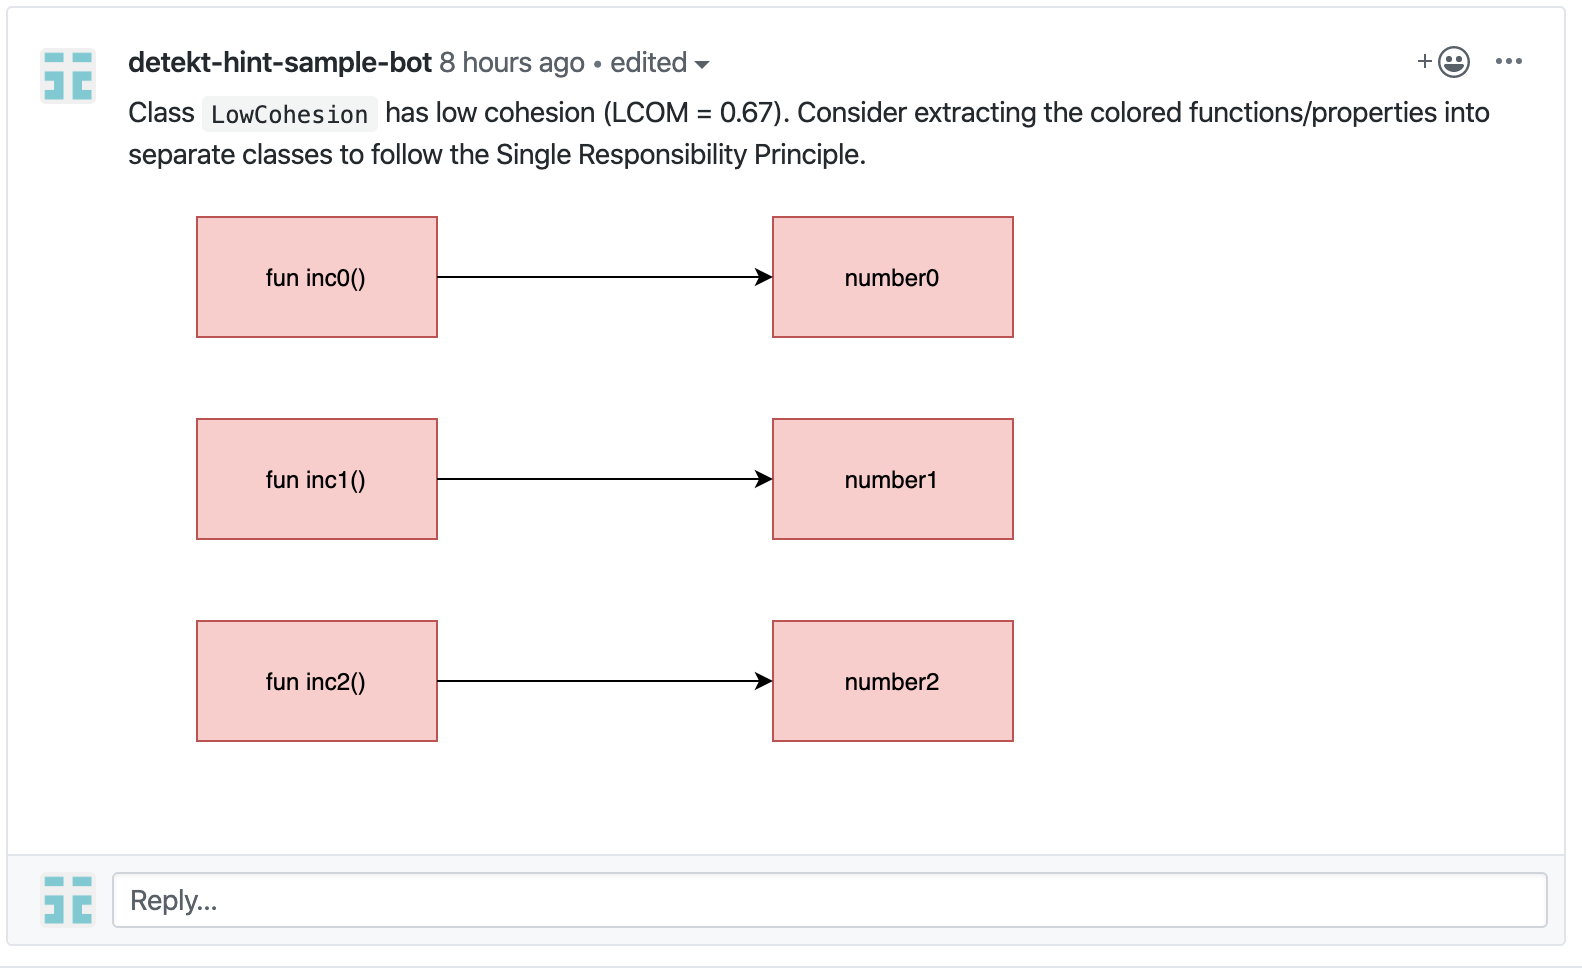
\includegraphics[width=\textwidth]{../images/comment_lackOfCohesion.png}
    \caption{Screenshot of the horizontal prototype showing the \gls{lcom} rule, with a visual representation of the lack of cohesion. The figure shows which fields that are referenced from each of the methods in the class. In this case all the methods of the class references their own separate field. This indicates that each of the methods and corresponding fields have separate responsibilities within the class. This would therefore be an indication of violating the \gls{srp}.}
    \label{fig:lcom}
\end{figure}


\begin{figure}[h!]
    \centering
    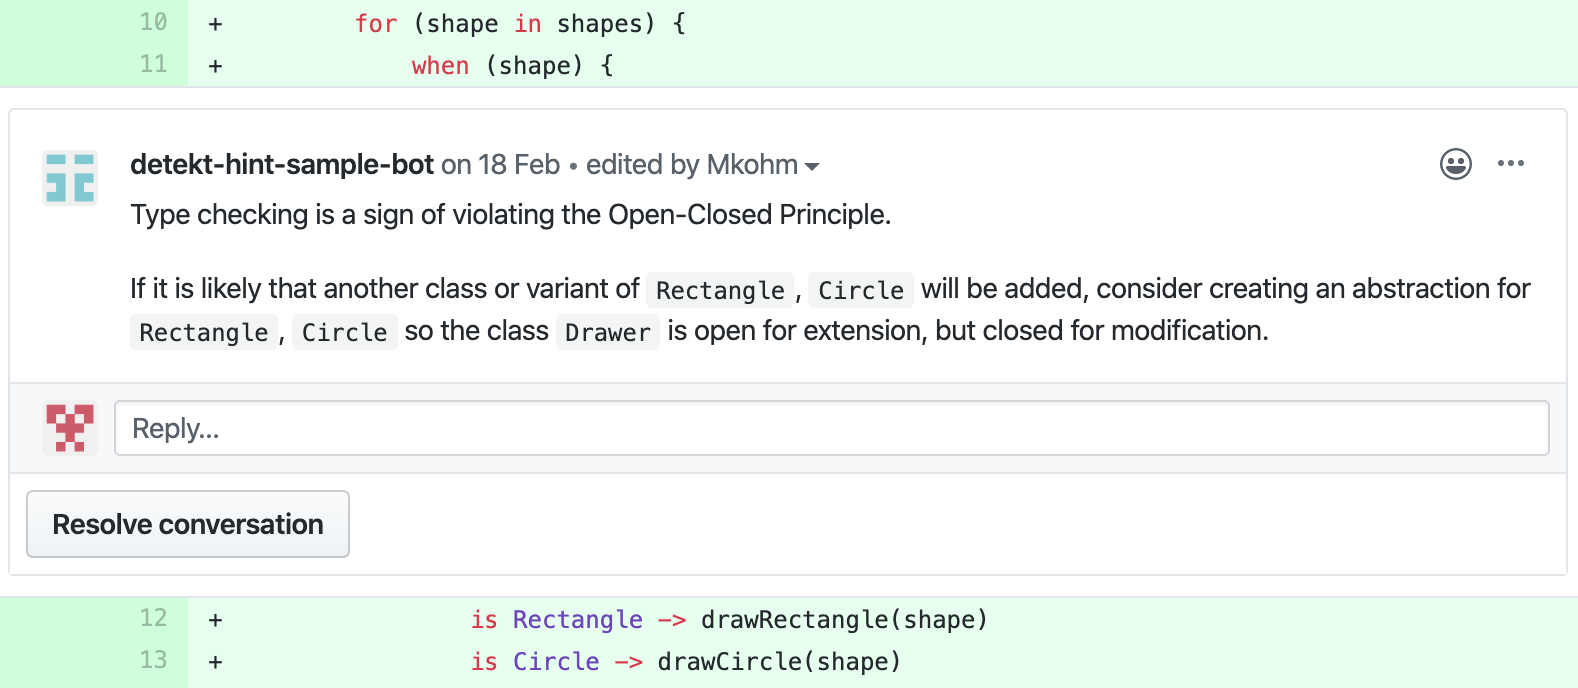
\includegraphics[width=\textwidth]{images/comment_ocp2.png}
    \caption{Screenshot of the horizontal prototype that shows the \gls{ocp} rule, using a simple program for drawing shapes. In this case the rule detected checking of concrete implementations to control flow. The rule suggests creating an abstraction for \texttt{Rectangle}, \texttt{Circle} (e.g an interface \texttt{Shape} with a \texttt{draw} method that all \texttt{Rectangle} and \texttt{Cirle} should implement) such that eventual new shapes added to the program would not need to modify existing code. }
    \label{fig:ocp}
\end{figure}


\begin{figure}[h!]
    \centering
    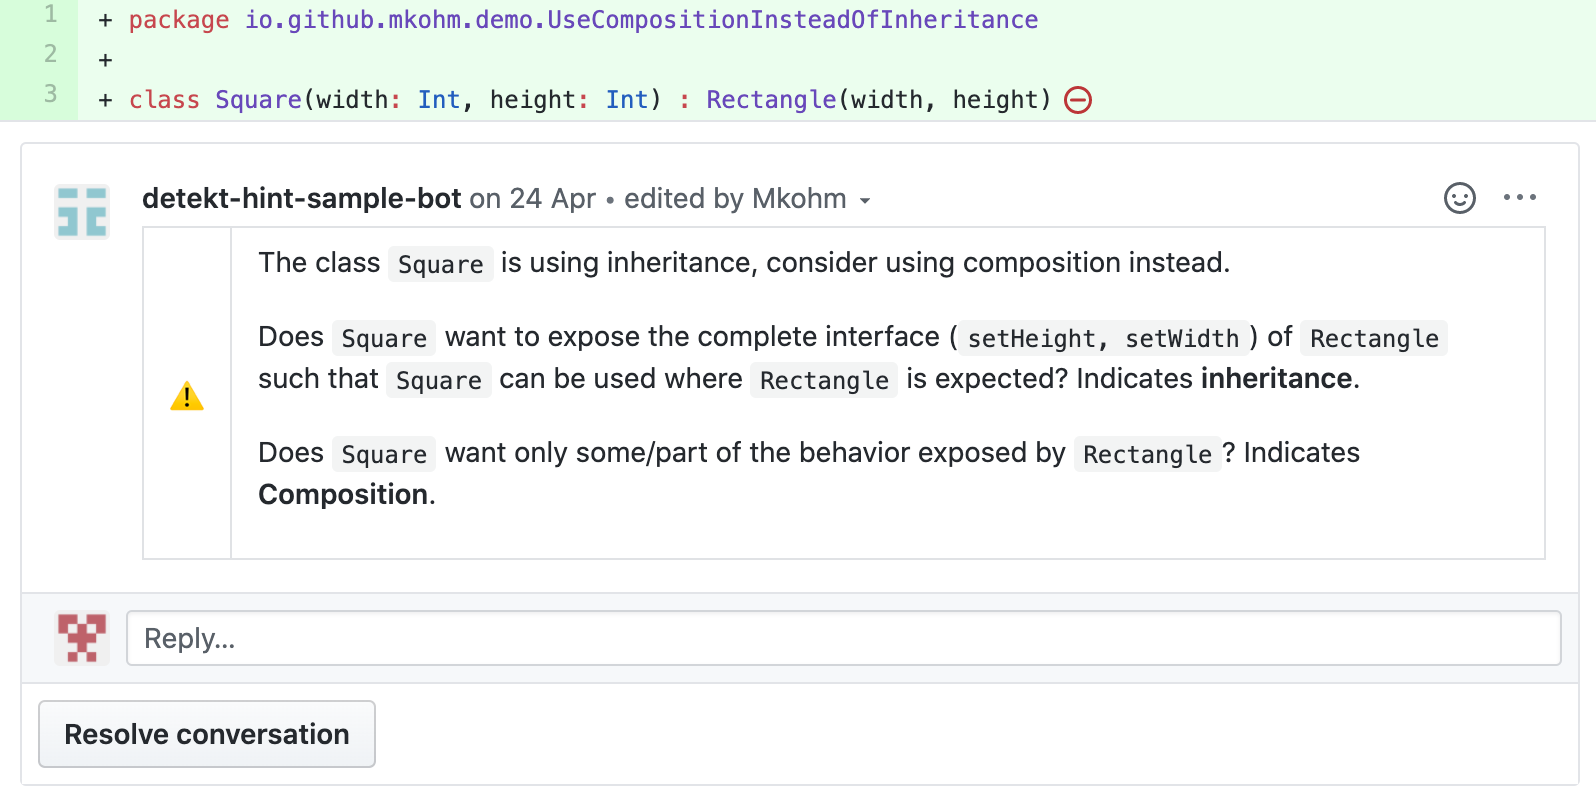
\includegraphics[width=\textwidth]{images/horizontal-prototype-coh.png}
    \caption{Screenshot of the horizontal prototype that shows the \gls{coi} rule. The rule suggests the use of composition instead of inheritance, and helps testing if the classes adheres to the \gls{lsp}. In this case, the classical Square - Rectangle problem is presented. \texttt{Square} should not be derived from \texttt{Rectangle} as it would violate the \gls{lsp}. \texttt{Square} does not functionally behave like \texttt{Rectangle} as squares by definition have the same width and height. \texttt{Rectangle} should have two independent methods for changing its size, but clearly these methods is not appropriate for the \texttt{Square}. }
    \label{fig:liskov}
\end{figure}

\clearpage

\section{Semi-structured interview schema}
\label{semi-structured-interview-schema}
\subsubsection*{Participant number:} What is the number of the participant.
\subsubsection*{Background:} What is the participants background. Experience with software architecture? Knows and uses design principles? Experience with Kotlin?
\subsubsection*{Presentation of rules - For each rule}
\begin{enumerate}
    \item Present the rule. 
    \item Make sure the participant understands the importance of the rule.
    \item When will the rule give a warning?
    \item When will the rule incorrectly give a warning? Will it report false-positives too often? Suggestions on how to reduce the amount?
    \item How much context is needed? Shorter or longer comments? Should include suggestions on possible solutions? Is the comment understandable? Something missing?
\end{enumerate}

\subsubsection*{Other} 
- When reviewing code, what do you think is tedious, and could it be automated?
- Are there any rules/principles missing?

\clearpage
\section{Semi-structured interview results}
\label{horizontal-prototype-interview-results}

\textbf{Participant number:} 1 \newline
\textbf{Background:} Studies computer science at \gls{ntnu} with a specialization in computers and systems software. Has experience with developing apps for iOS and web and back-end development. Interested in Software Architecture and writing software of high quality. \\
\textbf{Experience with design principles:} Some \\\\

\noindent \gls{coi}: Could be useful, but potentially have too many false positives. For testing the participant often creates Mock objects that inherits from the class he wants to Mock, and then overrides methods. The participant think there is too few cases where this rule will be useful. Suggestions: Reduce the amount of positives by disabling checks for classes with names; Mock. User could specify which class names or a pattern to ignore. Should revisit sentence number two about composition, it could be misleading.\\\\

\noindent LCOM1: Very useful because calculating such a value is'nt something you do while coding. Positive that you can change the threshold of the rule. Suggestion: Which fields and methods could i extract? A comment that suggests a solution. \\\\

\noindent LCOM2 (With refactoring visualization): Look more at further analysis to find out what can be extracted. Look into dependencies between function calls as well. Diagram looks cool, but does not give any more value than some plain text explaining what can be extracted. \\\\

\noindent \gls{ocp}: Somewhat useful. Should have a more specific comment saying if you are doing enum switching or instanceOf checking. \\\\

\noindent \gls{isp}: Could be useful. Suggestion to count number of usages of calls in the interface to see which method calls that is not used by any of the classes that implement the interface. \\\\

\noindent Other: Tools for detecting complicated expressions that can be extracted out as a separate method with a descriptive name. Blocks of code should be extracted out as separate methods so that lines of code that belongs together has its own scope. 
\clearpage


% Netlight
\noindent\textbf{Participant number:} 2 \newline
\textbf{Background:} Works as a software developer for Netlight, 2 years of professional developer experience. Experienced with Kotlin development and with architecture and design of software systems.\\
\textbf{Experience with design principles:} Yes \\\\

\noindent \gls{coi}: Positive about the rule, but is concerned about not showing warnings when deriving from third party libraries. This is a case where one also should think about using composition instead of inheritance. Suggests to remove this logic, and instead provide configuration options for packages that should not be reported as violations when derived from.  \\\\

\noindent \gls{lcom}: Nothing special. \\\\

\noindent \gls{ocp}: Useful for both instance of checking and enum switching. Enums in Kotlin are powerful, so switching on them is in many cases not needed and polymorphism is used instead.\\\\

\noindent \gls{isp}: Could be useful. May need to handle TODO's specially. \\\\

\noindent Other: In general positive to the tool, and think it has potential. Good that it is easy to ignore warnings, with just a click. It needs more rules before considering using it. For example including detection of Java anti-patterns and ensuring that Kotlin code is idiomatic. For example static methods and places where data-classes could be used. The tool could be used as "training wheels" in a team, where one gradually could disable more rules to not create unnecessary noise in the development.

\clearpage
\section{Final prototype}
\label{final-artifact}
\begin{figure}[h!]
    \centering
    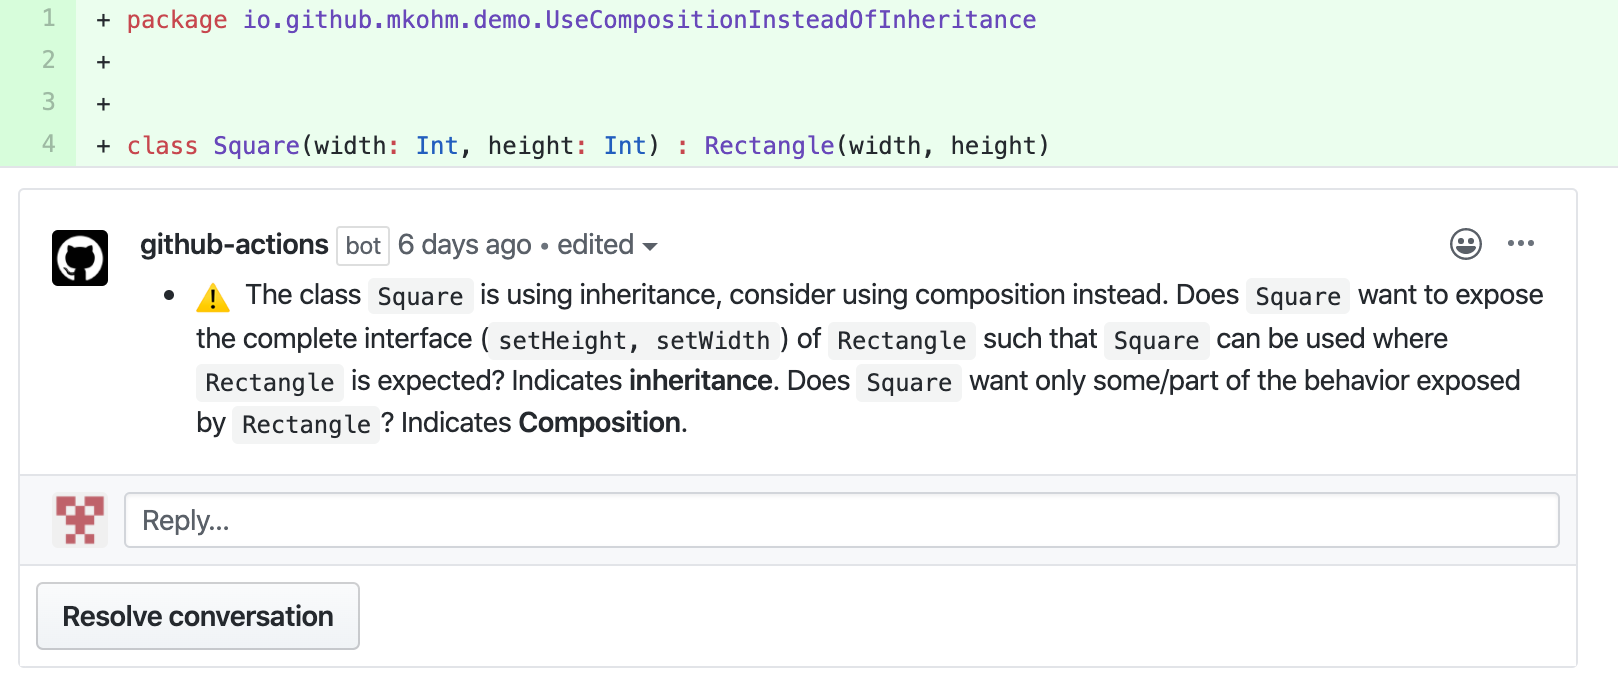
\includegraphics[width=\textwidth]{images/final_coh.png}
    \caption{Screenshot of the final prototype that shows the \gls{coi} rule. The rule suggests the use of composition instead of inheritance, and helps testing if the classes adheres to the \gls{lsp}. In this case, the classical Square - Rectangle problem is presented. \texttt{Square} should not be derived from \texttt{Rectangle} as it would violate the \gls{lsp}. \texttt{Square} does not functionally behave like \texttt{Rectangle} as squares by definition have the same width and height. \texttt{Rectangle} should have two independent methods for changing its size, but clearly these methods is not appropriate for the \texttt{Square}.}
\end{figure}

\begin{figure}[h!]
    \centering
    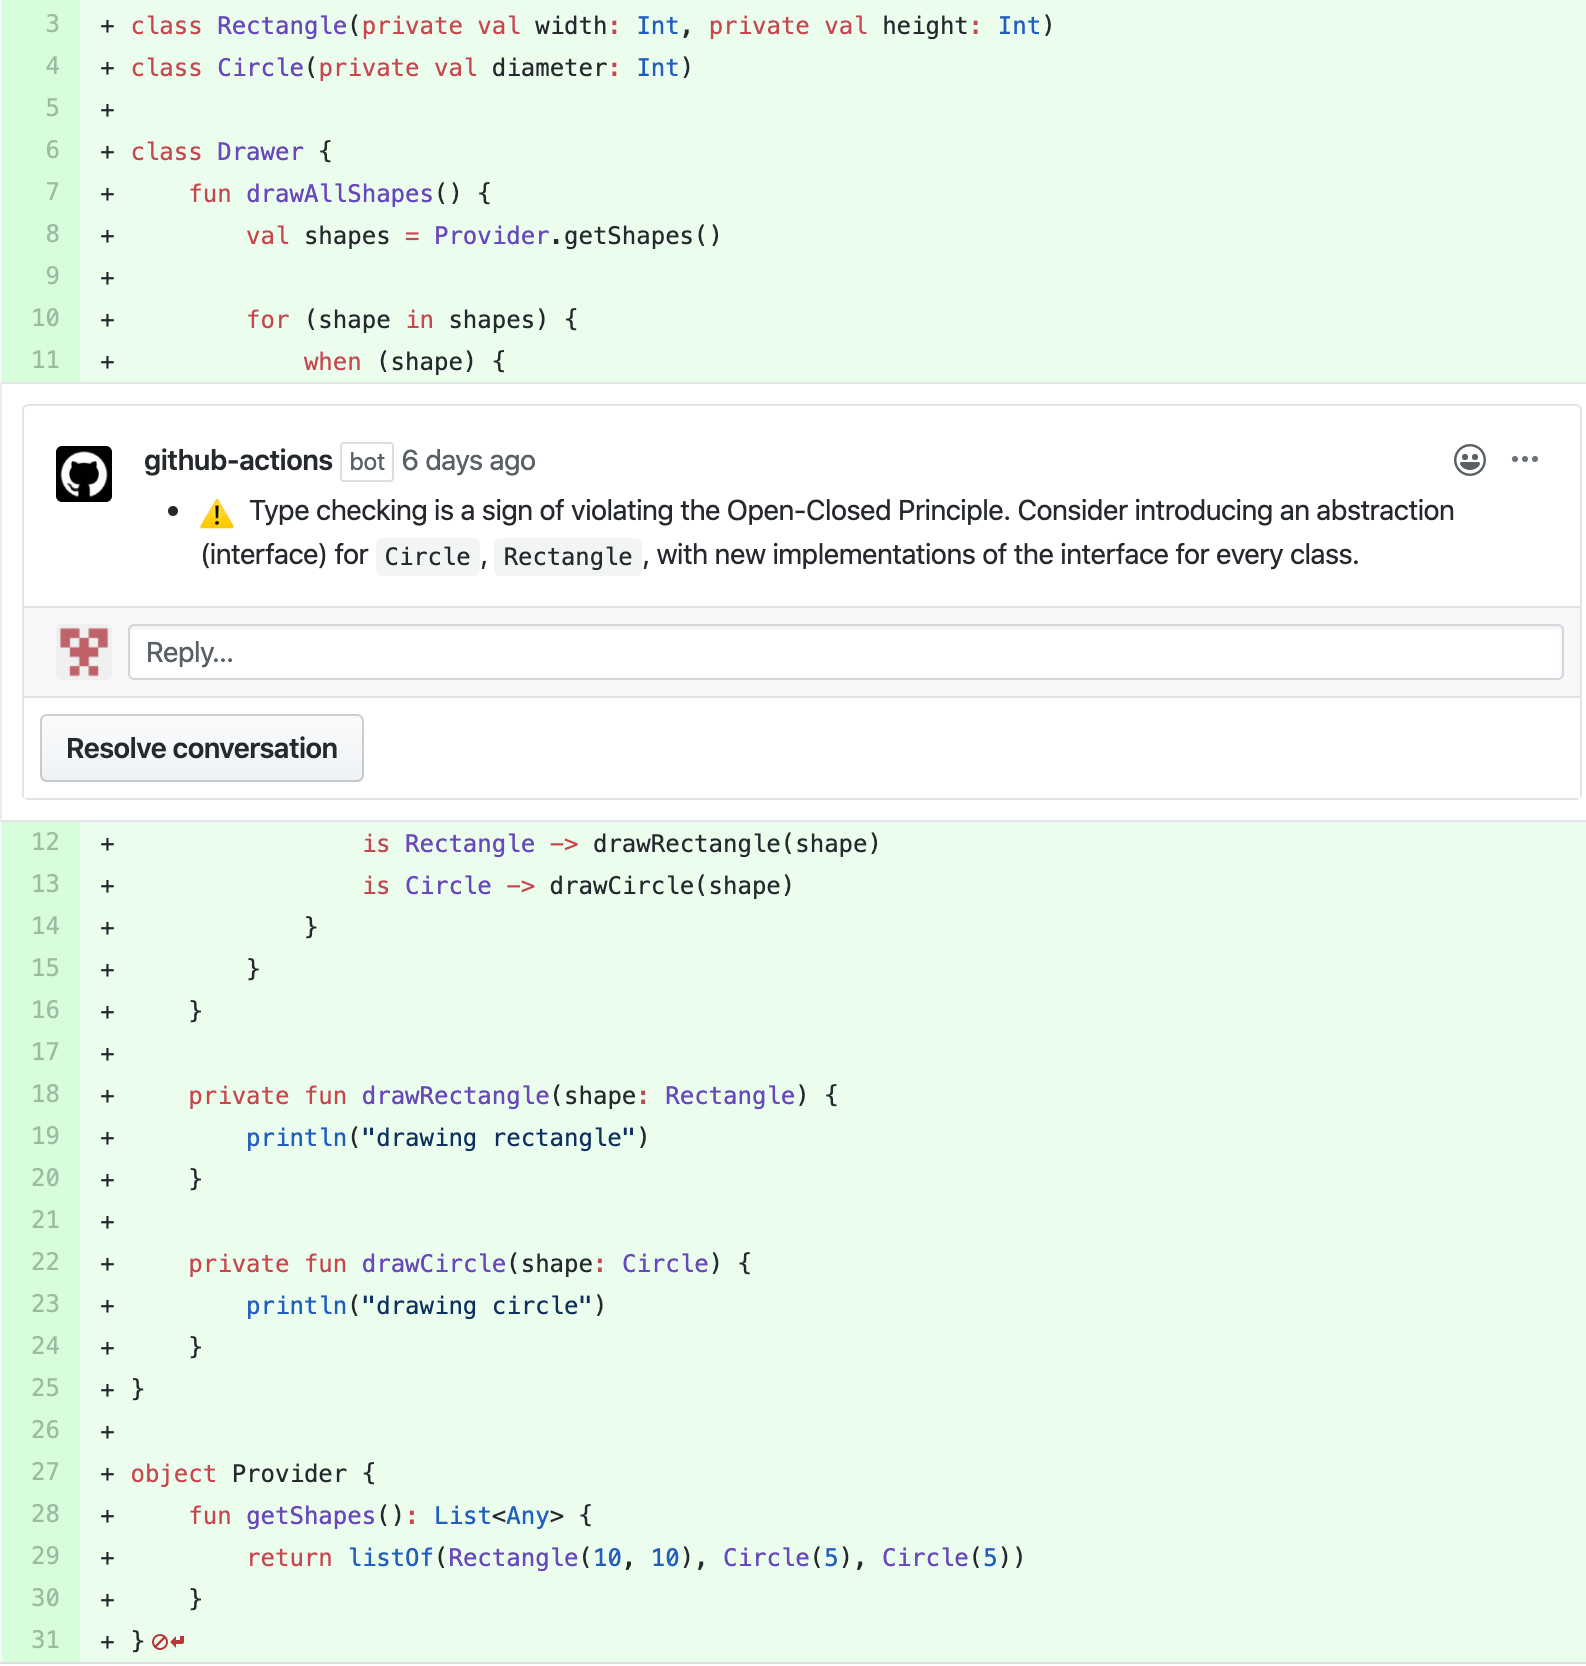
\includegraphics[width=\textwidth]{images/final_ocp.png}
    \caption{Screenshot of the final prototype that shows the \gls{ocp} rule, using a simple program for drawing shapes. In this case the rule detected checking of concrete implementations to control flow. The rule suggests creating an abstraction for \texttt{Rectangle}, \texttt{Circle} (e.g an interface \texttt{Shape} with a \texttt{draw} method that all \texttt{Rectangle} and \texttt{Cirle} should implement) such that eventual new shapes added to the program would not need to modify existing code.}
\end{figure}

\begin{figure}[h!]
    \centering
    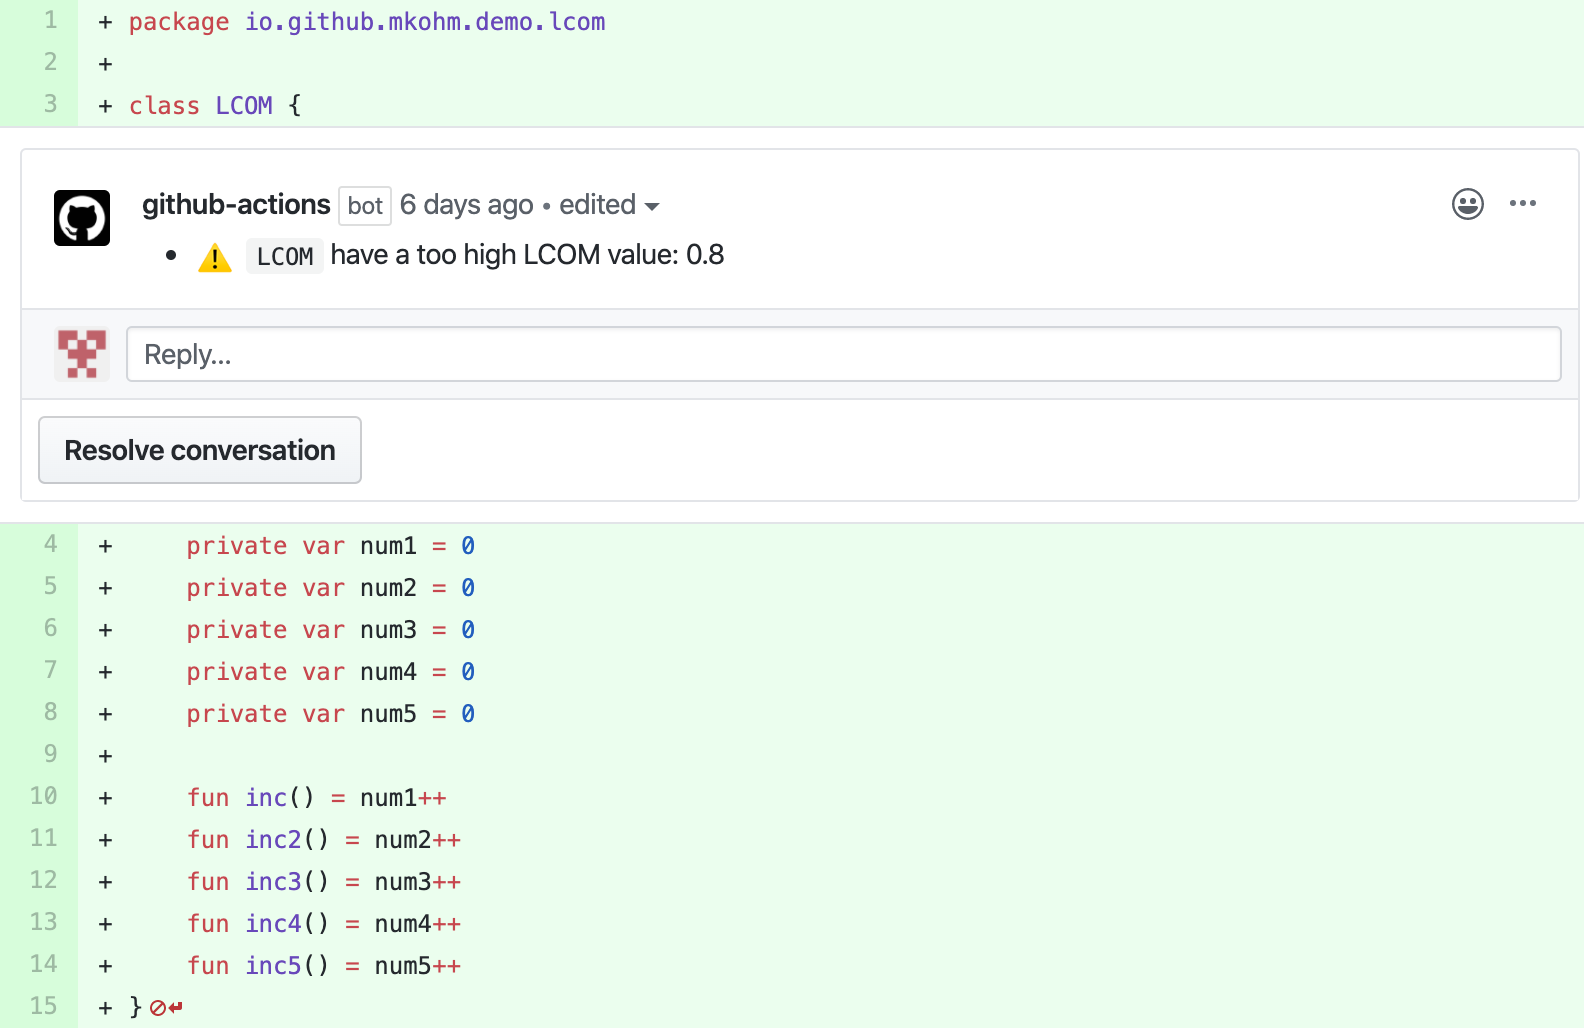
\includegraphics[width=\textwidth]{images/final_lcom.png}
    \caption{Screenshot of the final prototype showing the \gls{lcom} rule. This is an indication of violating the \gls{srp}, due to low cohesion in the class. In this case, each of the methods reference their own field, telling us that there is no relationship between the different methods, and that they don't need to exist in the same class.}
\end{figure}

\begin{figure}[h!]
    \centering
    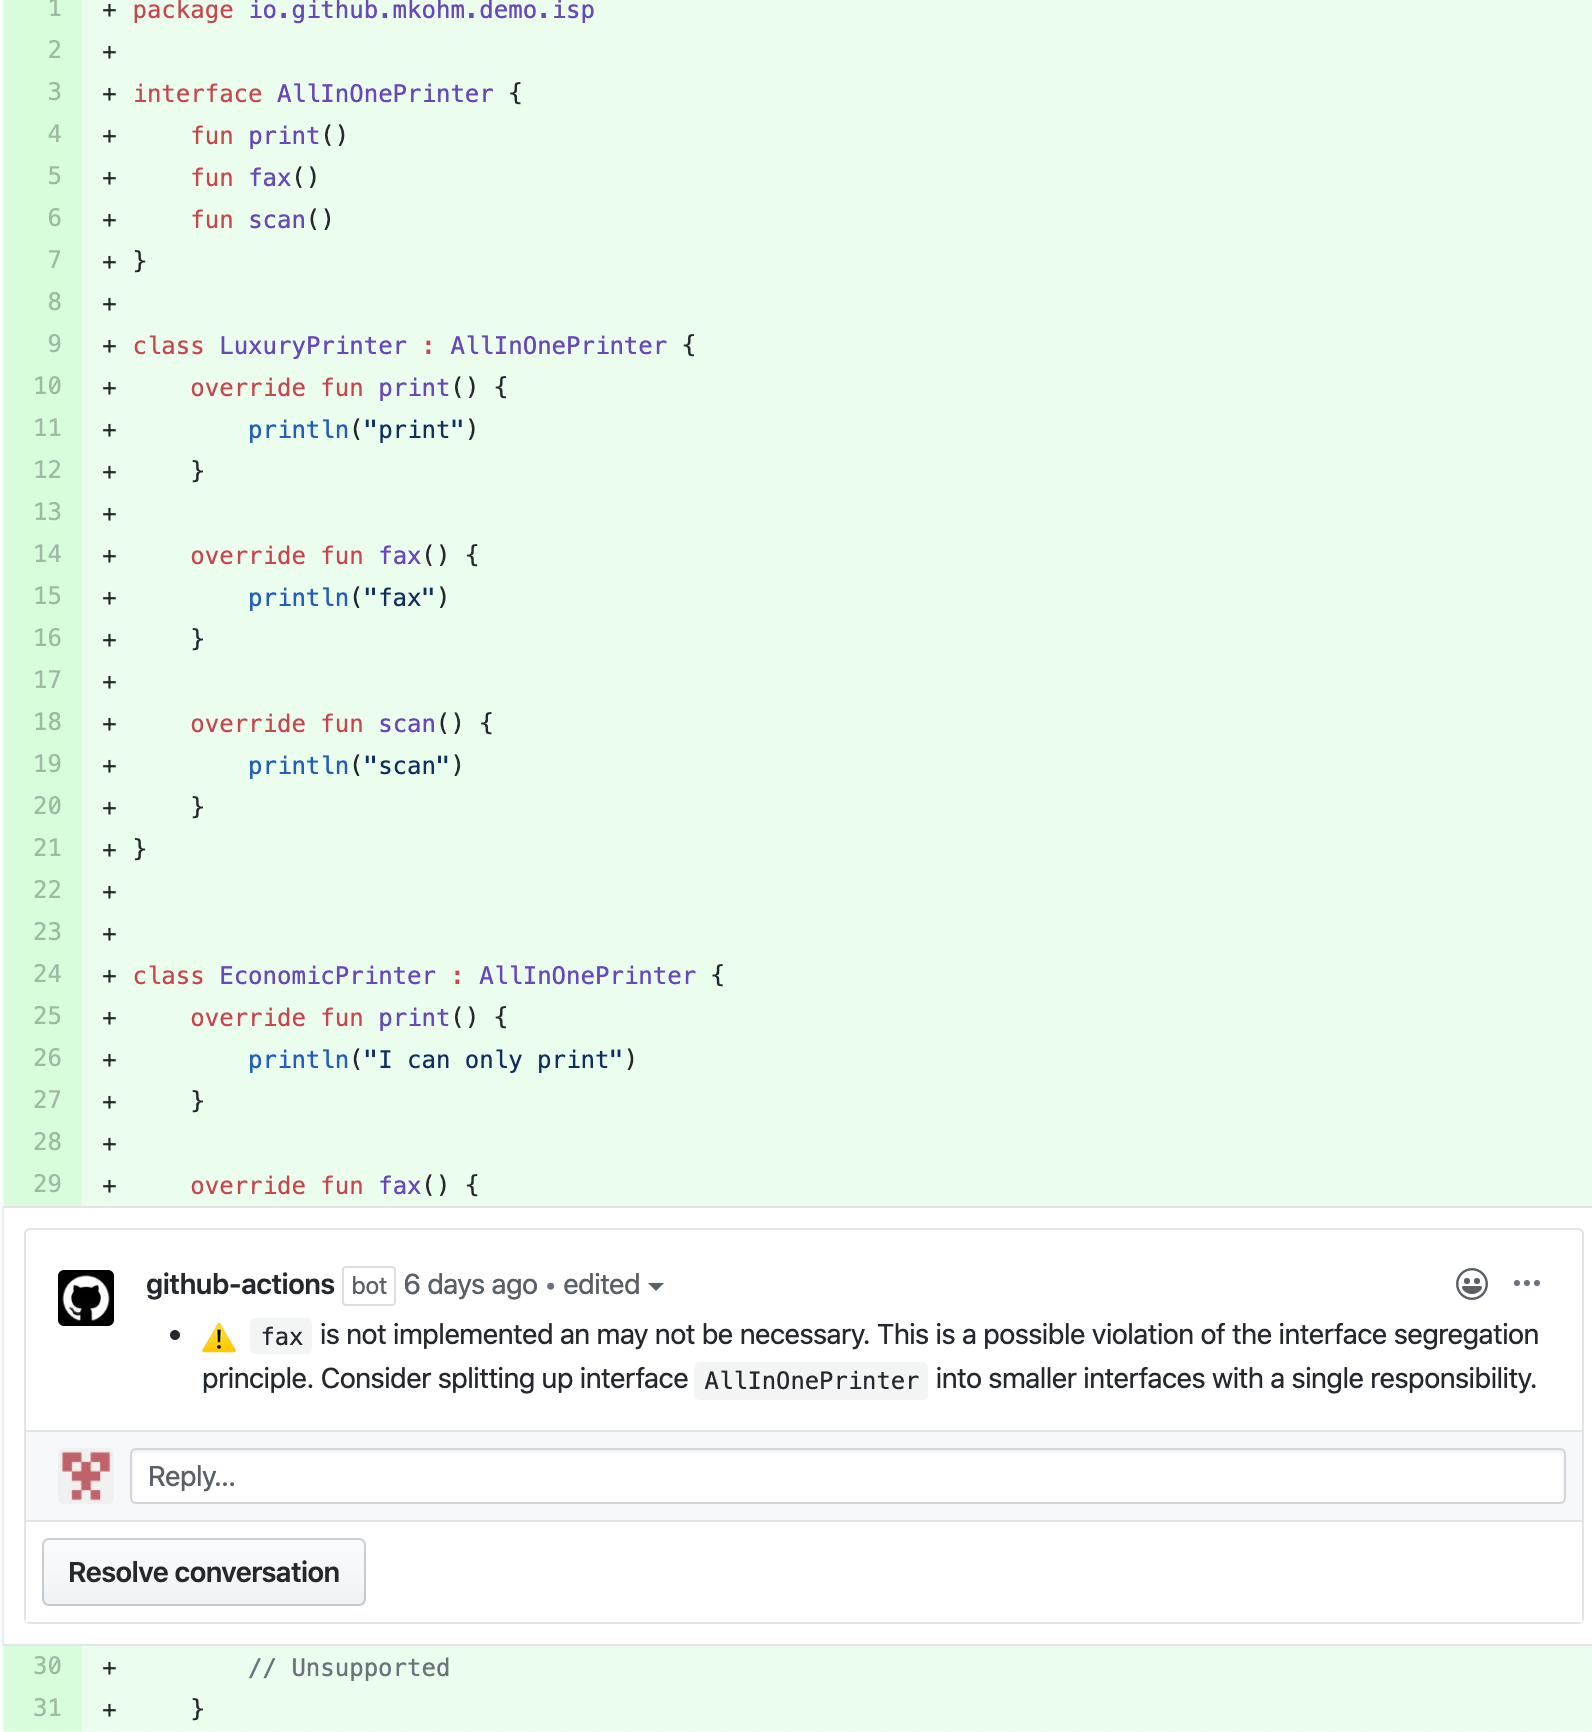
\includegraphics[width=\textwidth]{images/final_isp.png}
    \caption{Screenshot of the final prototype showing the \gls{isp} rule. It has detected an empty method, which is a sign of violating the \gls{isp}. In this case the \texttt{EconomicPrinter} implements methods from \texttt{AllInOnePrinter} which it does not need. A solution would be to define separate interfaces for each of the responsibilities (e.g \texttt{Printable, Faxable, Scanable}) and let the concrete implementations of printers implement the interfaces they need.}
\end{figure}

\end{document}